% Document template based on LNCS, adapted by Matt Welsh <mdw@cs.berkeley.edu>

% This version is adapted to use PDFTEX to render to PDF directly. 
% If you want to use dvi, you need to change any figures to use '.eps'
% rather than '.pdf', and probably get rid of the hyperref package.

% 03 Jan 2005 : GWA : Only standard option is conference format.

%\documentclass[10pt, conference, A4]{IEEEtran}
%\usepackage{program}
%\usepackage{times}  % Use Adobe Times font set
%\usepackage{epsfig,twocolumn}
%\usepackage{url}
%\usepackage[english]{babel} % mdw: Required to get good hyphenation on RH6.0
                            % (fixed in RH6.1)
%\usepackage{graphicx} 
%\usepackage{color}
%\usepackage{subfigure}

\documentclass[11pt, conference]{IEEEtran}
\usepackage{program}
\usepackage{times}  % Use Adobe Times font set
\usepackage{epsfig,graphicx}
\usepackage{url}
\usepackage[english]{babel}
\usepackage{color}
\usepackage{subfigure}

% 03 Jan 2005 : GWA : I think that this is what we want...
\usepackage{cite}

\newcommand{\XXXnote}[1]{{\bf\color{red} XXX-MDW: #1}}

\pagestyle{empty}
\begin{document}

%don't want date printed
\date{}

%%%%%%%%%%%% THIS IS WHERE WE PUT IN THE TITLE AND AUTHORS %%%%%%%%%%%%

% 03 Jan 2005 : GWA : Changed to use IEEE formatting.

\title{ Monitoring Volcanic Eruptions with a \\ Wireless Sensor Network}
\def\footnotemark{}

\author{\authorblockN{Geoffrey Werner-Allen\authorrefmark{1}, Jeff
Johnson\authorrefmark{2}, Mario Ruiz\authorrefmark{3}, Jonathan
Lees\authorrefmark{3}, and Matt Welsh\authorrefmark{1}}
\authorblockA{\authorrefmark{1}Harvard
University\\\{werner, mdw\}@eecs.harvard.edu}
\authorblockA{\authorrefmark{2}University of New
Hampshire\\jeff.johnson@unh.edu}
\authorblockA{\authorrefmark{3}University of North Carolina\\\{mruiz,
leesj\}@email.unc.edu}}

\thanks{For more information, please see: \\
{\tt http://www.eecs.harvard.edu/\~{}werner/projects\\/volcano}}

\maketitle

\thispagestyle{empty}

%%%%%%%%%%%%%  ABSTRACT GOES HERE %%%%%%%%%%%%%%

\begin{abstract}
This paper describes our experiences using a wireless sensor
network to monitor volcanic eruptions with low-frequency acoustic
sensors. We developed a wireless sensor array and deployed it in July 2004 at
Volc\'{a}n Tungurahua, an active volcano in central Ecuador.
The network collected infrasonic (low-frequency
acoustic) signals at 102~Hz, transmitting data over a 9~km wireless
link to a remote base station. During the deployment, we collected
over 54~hours of continuous data which included at least 9~large
explosions. Nodes were time-synchronized using a separate GPS
receiver, and our data was later correlated with that acquired at a
nearby wired sensor array. In addition to continuous sampling, 
we have developed a distributed event detector that automatically
triggers data transmission when a well-correlated signal is received
by multiple nodes. We evaluate this approach in terms of reduced
energy and bandwidth usage, as well as accuracy of infrasonic
signal detection.
\end{abstract}

%%%%%%%%%%%%%  BODY OF PAPER GOES HERE %%%%%%%%%%%%%%

\chapter{Introduction}
\label{chap-intro}

An emerging application for wireless sensor networks is their use in medical
care. Many medical applications place new demands on sensor network designs.
They often involve variable data rates, multiple receivers, and mobile
nodes. Most existing sensor network designs do not adequately support these
requirements, focusing instead on aggregating small amounts of data from nodes
at fixed locations. Therefore a gap exists between existing sensor network
architectures and the requirements of medical applications.

In this dissertation, we bridge the gap by making three contributions: we
propose CodeBlue medical sensor network architecture, TinyADMR ad-hoc multicast routing protocol, and LiveNet passive monitoring infrastructure.
With CodeBlue, we address the challenges of providing a flexible 
and implementable system architecture for mote-based medical
sensor networks. TinyADMR addresses challenges in multicast routing with the
existence of low quality radio links, memory and bandwidth limitations.
LiveNet addresses the challenges for evaluating deployed medical sensor
networks by reconstructing network dynamics without introducing additional
overhead to the network. We evaluate CodeBlue, TinyADMR and LiveNet
with an indoor sensor network testbed and with a disaster drill deployment.

\section{Medical sensor networks}

The convergence of several new hardware technologies, including MEMS, low
power processors, and low power radio, has enabled a new class of computing
platform: wireless sensors. Wireless sensors combine the capability of
sensing, computation, and wireless communication into a single physical
package, enabling a wide range of applications. Over the past decade, sensor
networks research community has explored the use of wireless sensors in
military target tracking and environmental monitoring such as habitats,
forests, volcanoes, civil infrastructures, factory equipments, and home energy
usage.

One common characteristic of most conventional sensor networks is that they
are intended for deployments of stationary nodes that transmit data at
relatively low rates, with a focus on best-effort data collection at a central
base station. Although the sensor networks research community has made
tremendous progress in perfecting networking and operating system support in
this space, we argue that there is a lack of adequate architectural
support for one emerging and important application domain: medical care.

In a hospital or clinic, outfitting every patient with tiny,
wearable wireless vital sign sensors allows doctors, nurses and other
caregivers to continuously monitor the status of their patients.  In
an emergency or disaster scenario, the same technology would enable
medics to more effectively care for large numbers of casualties.
First responders could receive immediate notifications on any changes
in patient status, such as respiratory failure or cardiac arrest.
Wireless sensors can augment or replace existing wired telemetry
systems for many specific clinical applications, such as physical
rehabilitation or long-term ambulatory monitoring.

A typical scenario involves many patients wearing sensors that monitor basic
vital signs such as heart rate or blood oxygen saturation. A small number of
medical personnel are responsible for continuously monitoring the patients
using devices such as laptops or PDAs. Using the real-time information
retrieved from the network, the medical team can treat
patients who need urgent care more efficiently.


\subsection{Application requirements}

Medical sensor networks have several different characteristics than
conventional sensor network applications. The sensors are worn by patients and the
data sinks are mobile computers carried by doctors or nurses so that the nodes
in the network are not stationary. Unlike typical sensor networks, there are
likely to be more than one data sinks in the network. Nodes can also join or
leave the network dynamically. Furthermore, the data traffic pattern is
on-demand and dynamic. Different doctors may be interested in real-time status
of different groups of patients and the groups can potentially overlap. There may
also be interests for different types or resolutions of sensor data.
Conventional sensor network architectures are inadequate in such scenarios
because the system cannot assume fixed sensor queries, sampling rate and
static traffic pattern. 


%% data may have different priorities associated with it

\subsection{Resource limitation}

In addition to meeting a different set of application requirements, medical sensor
networks, as conventional sensor network systems, face the challenges from
severe
resource limitations of the low power sensor platforms. To be practical, the
sensor nodes must be light-weight, low power and low cost so that they can be
wearable, have long enough battery lifetime and be affordable. This entails
the use of low power radio and low power processor.  For example, the mote
platform, MicaZ~\cite{micaz}, that we use for our medical sensor networks has
4~KB of RAM, a 4~MHz 8-bit CPU and a low power IEEE 802.15.4 radio with
maximum transmit power at 0 dBm. The implication of such a limited platform is
that the software running on the mote cannot be overly computationally
intensive or require large amount of memory. Yet, the system must be responsive enough
to handle complex
interactions with the environment such as sampling medical sensors and
performing radio communication in time. As a result, we not only have to find
a new architecture that fulfills the application requirements, it must also be
designed carefully so that it is light weight enough to fit into the platform
but complex enough to fulfill the application demands. 

\section{Systems challenges for medical sensor networks}

We outline a set of challenges identified through the process of designing,
implementing, deploying, and evaluating a medical sensor network. First of
all, there needs to be a new network architecture to efficiently support the
type of queries and traffic patterns for medical sensor networks. Secondly,
to support the new architecture, it is necessary to provide multicast routing
capability on resource-limited sensor nodes. Third, studying a deployed
medical sensor network requires a non-trivial network monitoring infrastructure.

\subsection{A new network architecture}

In contrast to conventional sensor network applications, medical monitoring
must support a large number of patient sensors deployed in a hospital or
disaster site, a variety of data rates, and multiple mobile receiving
devices, such as PDAs carried by doctors or medics. Moreover, medical
monitoring cannot make use of traditional
in-network aggregation since it is not generally meaningful to combine data
from multiple patients. The goal is instead to efficiently deliver information
to the correct receivers. Therefore, there is a significant gap between
existing sensor network designs and the requirements of medical monitoring. 

Supporting such broad range of requirements demands a new approach to
sensor network design. To bridge the technology gap, we propose CodeBlue, an
architecture for medical sensor networks that provides a set of protocols and
services tailored for this application domain. CodeBlue includes
a publish/subscribe communication model, a rich query interface for periodic
and triggered collection of sensor data, a dynamic sensor discovery protocol,
and a programmatic external interface based on Web Services standards.
CodeBlue provides a high-level interface to the network, making it easy to
support new sensor types and applications that tie into real-time medical
sensor data.

\subsection{Multicast on resource limited sensor nodes}

By reviewing the application requirements of medical sensor networks, it
becomes clear that an ad-hoc multicast routing protocol is more adequate
than the conventional many-to-one data collection tree routing approach.
Fortunately there are existing multicast protocols designed for ad-hoc mobile
networks. However, after the attempt to implement one such protocol, ADMR, on
our resource limited sensor platform, we have discovered several challenges
that were not foreseen by the original designers. In order to achieve
acceptable packet delivery ratio, we have to use different routing metrics that
involves the use of link quality information. We have also
investigated the challenges to scale the network within the memory and
bandwidth limitations on the sensor platform.

\subsection{Deployment support}

To find out whether a design is practical for realistic use, one needs to
deploy the network and evaluate the performance in a realistic environment.
For this purpose, we have conducted a deployment study of the CodeBlue
network. It is necessary to record system behavior in order to study
the correctness and performance of the network during the deployment. Under severe
resource constraints on CPU, memory and bandwidth, it is not practical to
record such information on the sensor nodes locally or transmit the logged
information over the radio. To overcome this problem, we have designed and
built LiveNet, an entirely passive monitoring infrastructure for
reconstructing dynamics of deployed sensor networks.  LiveNet is passive and
therefore does not require changing the application code or incur any
additional resource consumption in the network. Yet, it is able provide
valuable information for evaluating and debugging the deployed network.

\section{Dissertation outline}

The remainder of the dissertation is organized as follows.

Chapter 2 considers background and related work. This chapter introduces 
existing work in sensor networks and ad-hoc networking research community that 
are related to medical sensor networks. We also provide an overview of target
hardware platforms of this thesis.

Chapter 3 presents the requirements for a large class of medical sensor
network applications and a new software architecture to meet these
needs. We first propose the CodeBlue network architecture by presenting the
system goals and overall architecture design. We then describe individual
components
to discuss the design trade-offs in detail. Our key contributions include
proposing publish/subscribe as the appropriate networking abstraction for
a medical sensor network and designing CodeBlue Query (CBQ) interface, which
provides a programmatic interface to the medical sensor network.

Chapter 4 presents our approach to achieving efficient publish/subscribe
communication in sensor networks with mobile nodes, based on the
ADMR~\cite{admr-mobihoc01} {\em ad-hoc\/} multicast routing
protocol. We first describe the challenges encountered when designing and 
implementing the multicast layer to support publish/subscribe communication 
model for CodeBlue. We identify the
challenges from unreliable wireless radio links, memory constraints and
bandwidth constraints. We also explore and evaluate different route discovery
and expiration strategies. The key contributions include two new 
routing metrics that exploit link quality information and identifying
scalability limitations from memory and bandwidth constraints.

Chapter 5 describes LiveNet passive monitoring infrastructure. This chapter 
covers the architecture of LiveNet that involves passive sniffers, trace
merging algorithm and a set of analyses that are used to analyze CodeBlue
deployments. We also present the results of an extensive validation study of 
LiveNet's performance and accuracy with a set of controlled experiments with 
an indoor testbed, MoteLab.

Chapter 6 covers implementation and detailed performance evaluation of
CodeBlue network architecture.  We present evaluation of CodeBlue both on a
sensor network testbed and with a disaster drill deployment.  The testbed
experiments evaluate CodeBlue in scalability, fairness, latency, jitter and
effect of mobility. Then we present a deployment study that was part of a disaster
drill simulating a bus accident. Using data from LiveNet, we are able to
analyze the traffic load, network hotspots, routing paths, and query yield for
this deployment.

Chapter 7 contains lessons learned from the experience of 
designing, implementing, deploying and evaluating medical sensor networks and
provide potential future research directions. 

Chapter 8 concludes.
 
\section{Background}
\label{evaluation-sec-background}


%\subsection{Previous work}

% Tungurahua and Reventador deployment
%Our group is one of the first to explore the use of low-power 
%wireless sensor networks for geophysical monitoring, particularly 
%on active volcanoes. Although wireless telemetry is used on 
%seismic arrays at dozens of volcanoes worldwide, such installations involve 
%large, power-hungry equipment that is not well-suited for rapid, 
%dense deployments. As a result, even many of the most most threatening 
%and active volcanoes (e.g., Mount St. Helens~\cite{malone-81}) maintain 
%networks of less than ten stations.
%One of the primary limitations of volcano seismological studies is simply
%the lack of spatial coverage on a particular volcano.  
%This is true of
%heavily-monitored volcanoes like Mt. St. Helens and Mt. Fuji as well as
%on remote locations in Ecuador.

%Our team has been collaborating for the last two years and has deployed
%two wireless arrays on volcanoes in Ecuador. Our first deployment in
%July 2004 at Volc\'{a}n Tungurahua demonstrated the proof-of-concept, 
%involving three wireless sensor nodes sampling continuous infrasonic 
%time series data~\cite{volcano-agu04,volcano-ewsn05}.  
%The sensor array transmitted continuous, real-time infrasonic signals to
%a base-station laptop via a radio modem 9~km from the deployment site.
%The network operated for 54~hours and collected data on a dozen
%eruptive events during this time. This deployment helped us to optimize
%node placement, packaging, and radio communication in a challenging
%environment. The second installation at Volc\'{a}n Reventador is the
%subject of this paper and is described in the next section.

%In this paper we focus on our second deployment in August 2005, 
%in which we deployed a larger, more sophisticated network on the 
%upper flanks of Volc\'{a}n Reventador. A previous magazine 
%article~\cite{volcano-ieeeic06} detailed the network architecture
%and an overview of the deployment itself. Briefly, the network 
%consisted of 16~nodes, each with seismometers and microphones, 
%distributed over a 3~km extent running radially from the vent. 


\section{System Architecture}
\label{evaluation-sec-design}

% 17 Apr 2006 : GWA : Brief overview of system design.  For now I'm going to
%               defer as many details as possible to the evalution sections
%               since we've covered this in some detail in the IEEE article.
%               Also trying to avoid recycling the wording.  I'm working from
%               the paper copy so the skeleton might be similar though.

In this section we provide a brief overview of the design of our volcano
monitoring sensor network and details of the deployment at Reventador. In an
earlier magazine article~\cite{volcano-ieeeic06} we describe the system and
deployment in more detail, although we have not previously published results
evaluating its performance.

\subsection{Sensor hardware}
\label{evaluation-sec-hardware}

\begin{figure}[t]
\label{evaluation-fig-station}
\begin{center}
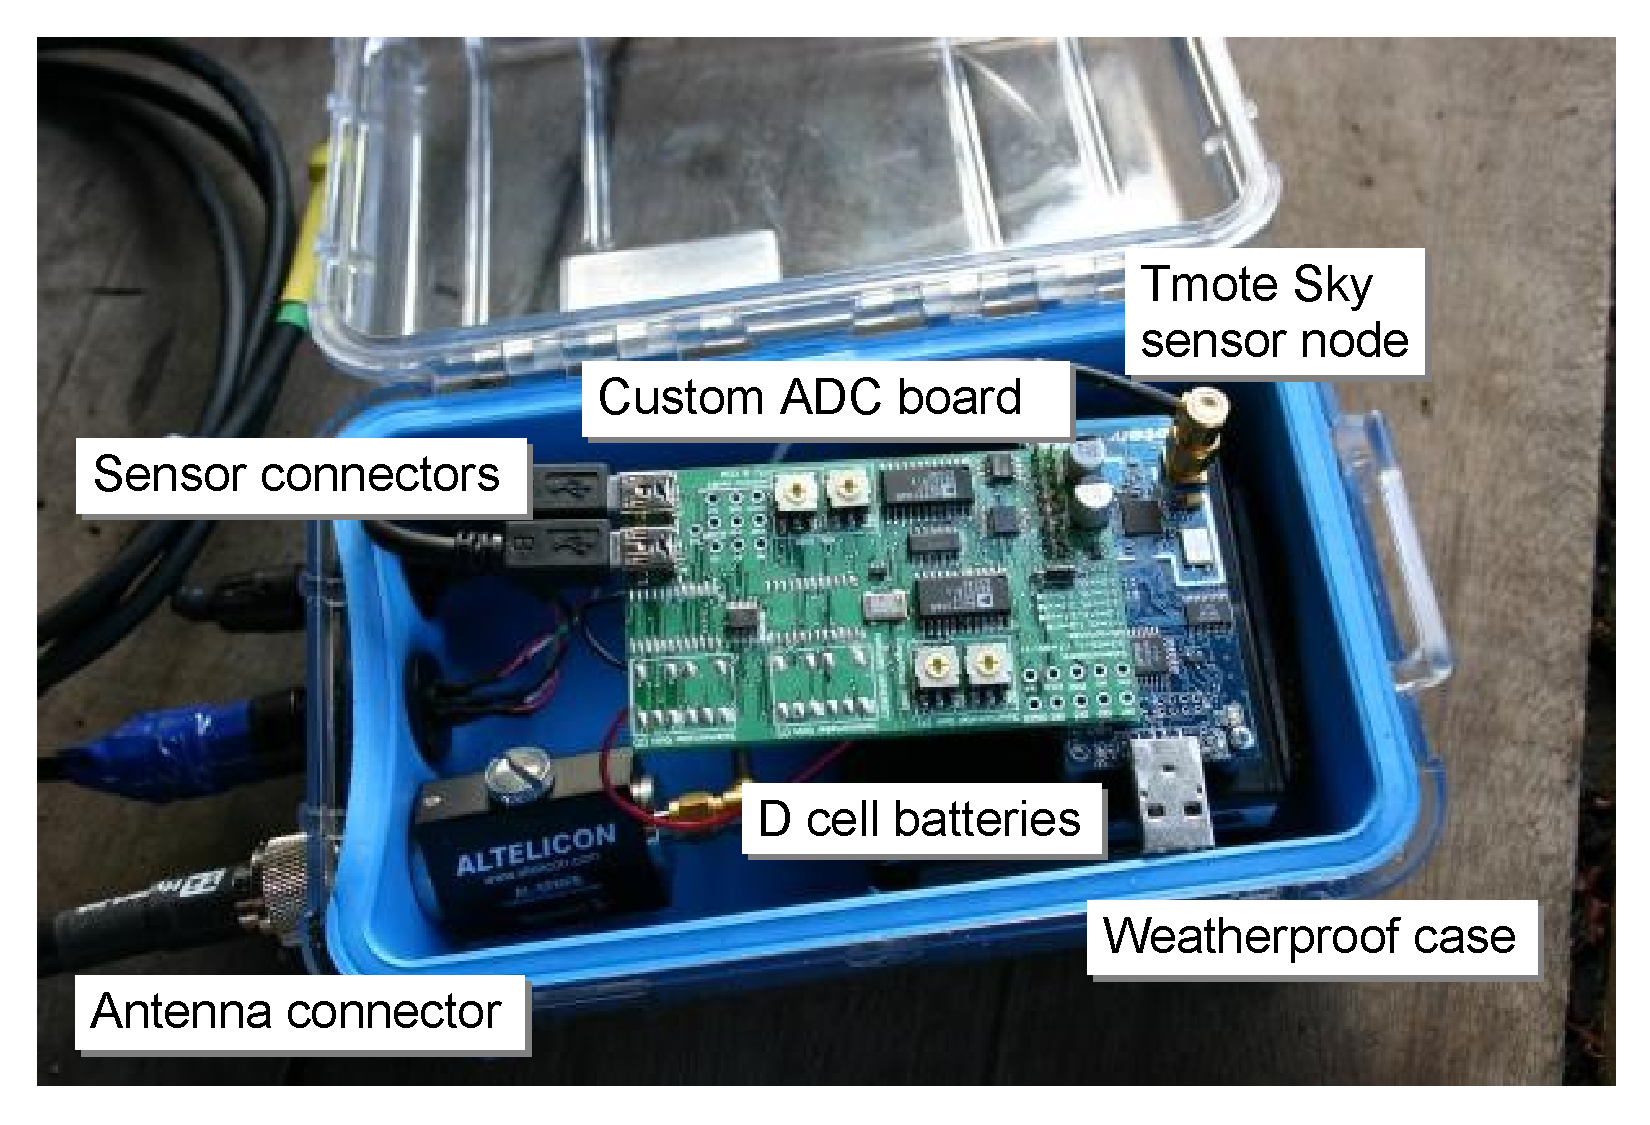
\includegraphics[width=1.0\hsize]{./5-evaluation/figs/pics/Station2-small.pdf}
\end{center}
\caption{\textbf{Our wireless volcano monitoring sensor node.}}
\end{figure}

%We deployed 16 wireless monitoring stations onto Volc\'{a}n Reventador.
%Nodes were arranged in a roughly-linear configuration radiating from the vent
%and spanning over 3km.  Figure REFERENCE shows the locations of each node as
%well as those of several wired monitoring stations deployed nearby.
%\GWAnote{Do we event want to include this figure again? It takes up a lot of
%space but it probably would be nice to have...}

Our wireless sensor node (Figure~\ref{evaluation-fig-station}) is based on
the TMote Sky~\cite{moteiv} platform, which integrates a TI~MSP430 processor,
10~KB of SRAM, 48~KB of program ROM, 1~MByte of flash memory, and a Chipcon
CC2420 radio. All software is implemented in TinyOS~\cite{tinyos-asplos00}.
We designed a custom sampling board that provides four channels of 24-bit
analog-to-digital conversion (TI~AD7710). 
%While the MSP430 provides several channels of ADC, its resolution of 16~bits
%was inadequate for our needs.

Nodes were interfaced to either a single-axis seismometer (GeoSpace GS-11) or
three seismometers in a triaxial configuration (GeoSpace GS-1). 
%The GS-11 sensors are inexpensive and lightweight, but are only sensitive at
%frequencies above 4.5~Hz. In contrast, the GS-1 sensors have a corner
%frequency of 1~Hz but are significantly more expensive and heavy. 
Both sensors are passive instruments; ground motion generates a voltage which
is amplified and digitized by the sampling board.  In addition, each node was
attached to an omnidirectional microphone (Panasonic WM-034BY). This
microphone has been used in other infrasonic monitoring
studies~\cite{johnson-etal-04b}.

% MDW: Node 204 talked to 206 which was 1055 meters away!
Each node was equipped with an 8.5~dBi omnidirectional antenna mounted on
1.5~m of PVC pipe.  This permitted line-of-sight radio range of over 1~km
without amplification; nodes were typically placed 200-400~m apart in our
deployment. Nodes were powered by two D-cell batteries with a lifetime of
approximately 1~week.  Each node was enclosed in a weatherproof Pelican case.

Several other pieces of hardware complete the system. FreeWave radio modems
provided a long-distance radio link between the sensor array and the volcano
observatory, 4.6~km away. A laptop located at the observatory logged data and
was used to monitor and control the network.  Finally, to establish a global
timebase, we used a single Crossbow MicaZ~\cite{xbow} mote interfaced to a
GPS receiver (Garmin OEM~18~LVC).  The GPS receiver provided a 1~Hz pulse
that is accurate to GPS time within 1~$\mu$s, and acted as the root of the
network time synchronization protocol as described in
Section~\ref{evaluation-sec-timing}.

\subsection{Network topology and status monitoring}

Nodes form a multihop routing tree rooted at the gateway node that is
physically attached to the FreeWave modem; we use a variant of
MintRoute~\cite{awoo-multihop} that uses the CC2420's Link Quality Indicator
metric to select routing paths. Each node transmits a {\em status message}
every 10~sec that includes its position in the routing tree, buffer status,
local and global timestamps, battery voltage, and other information. 
%These status messages form the basis of much of the analysis in this paper.
In addition, the base station can issue a {\em command} to each node,
instructing it to respond with an immediate status message, start or stop
data sampling, and set various software parameters.  Commands are propagated
using a simple flooding protocol.  The {\em Deluge} protocol~\cite{deluge}
was also used to permit over-the-air reprogramming and rebooting of nodes.

\subsection{Event detection and data collection}

Because of the high data rates involved (600-1200~bytes/sec from each node)
it is infeasible to continuously transmit all sensor data. Rather, nodes are
programmed to locally detect interesting seismic events and transmit event
reports to the base station. If enough nodes trigger in a short time
interval, the base station attempts to download the last 60~sec of data from
each node.  This design forgoes continuous data collection for increased
resolution following significant seismic events, which include earthquakes,
eruptions, or long-period (LP) events, such as tremor.  The download window
of 60~sec was chosen to capture the bulk of the eruptive and earthquake
events, although many LP events can exceed this window (sometimes lasting
minutes or hours).  To validate our network against existing scientific
instrumentation, our network was designed for high-resolution signal
collection rather than extensive in-network processing.
%In the future we would like to explore more advanced in-network signal
%processing.

During normal operation, each node continuously samples its seismic and
acoustic sensors at 100~Hz, storing the data to flash memory. Data is stored
as 256-byte {\em blocks} in the flash.
%with each block identified by a monotonically increasing {\em block ID}.
Each block 
%is tagged with its ID 
is tagged with the {\em local timestamp} corresponding to the first sample in
the block.  This timestamp is later mapped onto a global time reference as
described in Section~\ref{evaluation-sec-timing}. The 1~Mbyte flash is
treated as a circular buffer storing approximately 20~min of data. 

In addition, nodes run an {\em event detection algorithm} that computes two
exponentially-weighted moving averages (EWMA) over the input signal with
different gain settings. When the ratio between the two EWMAs exceeds a
threshold, the node transmits an event report to the base station.
%$\alpha_{\mathit{high}} > \alpha_{\mathit{low}}$.  That is, the high-gain
%EWMA is more sensitive to changes in the input signal than the low-gain
%EWMA. If the ratio of the high-gain EWMA to the low-gain EWMA exceeds a
%threshold $T$, the node considers the signal to contain a significant event
%and transmits a {\em trigger} message to the base station.
If the base station receives triggers from 30\% of the active nodes within a
10~sec window, it considers the event to be well-correlated and initiates
data collection.

Our reliable bulk-transfer protocol, called {\em Fetch}, operates as follows.
The base station waits for 30~sec following an event before iterating through
all nodes in the network. The base sends each node a command to temporarily
stop sampling, ensuring the event will not be overwritten by subsequent
samples.  For each of the 206~blocks in the 60~sec window, the base sends a
{\em block request} to the node.  The node reads the requested block from
flash and transmits the data as a series of 8~packets.  After a short timeout
the base will issue a repair request to fill in any missing packets from the
block.
%The repair process continues until all packets have been received or a
%timeout occurs. 
Once all blocks have been received or a timeout occurs, the base station
sends the node a command to resume sampling and proceeds to download data
from the next node. 
%The data is logged by the base station laptop for later analysis.

\subsection{Deployment on Volc\'{a}n Reventador}

\begin{figure}[t]
\label{evaluation-fig-schematic}
\begin{center}
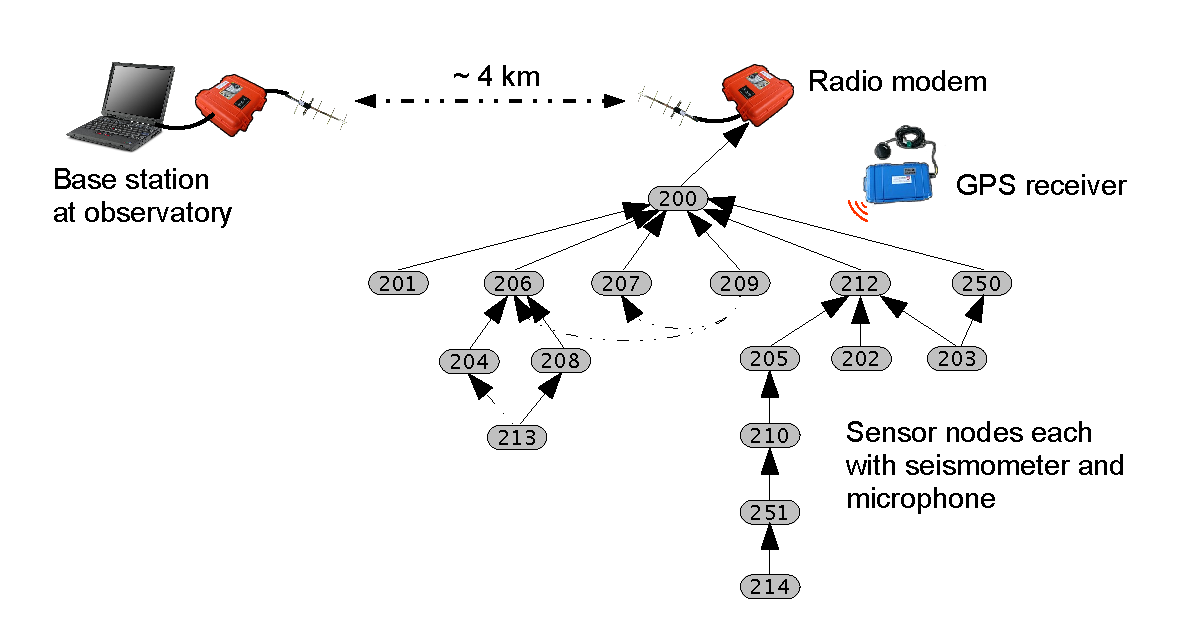
\includegraphics[width=1.0\hsize]{./5-evaluation/figs/pics/schematic2.pdf}
\end{center}
\caption{\textbf{Sensor network architecture.} Nodes form a
multihop routing topology, relaying data via a long-distance radio
modem to the observatory. A GPS receiver is used to establish a global
timebase. The network topology shown here was used during
our deployment at Reventador.}
\end{figure}

\begin{figure}[t]
\label{evaluation-fig-map}
\begin{center}
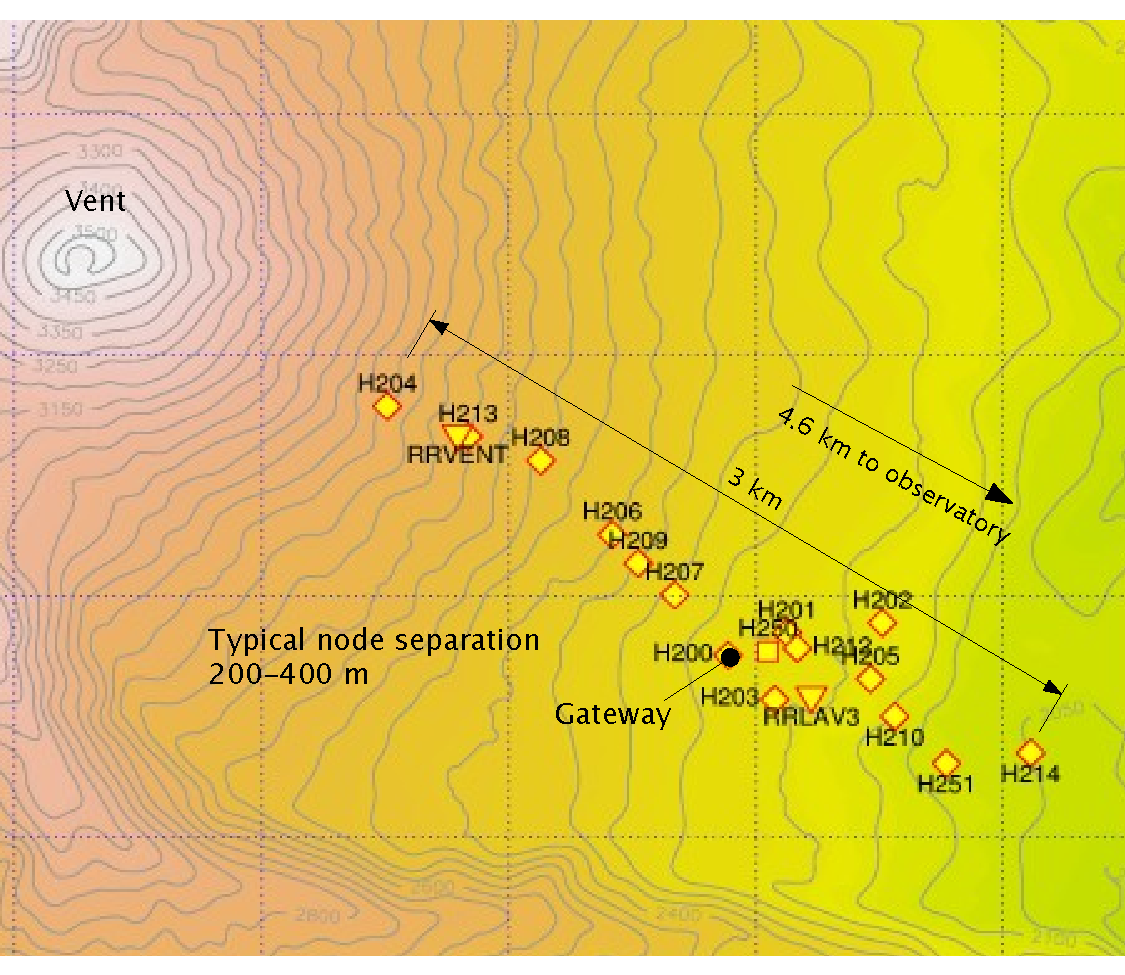
\includegraphics[width=1.0\hsize]{./5-evaluation/figs/pics/reventador-map-crop.pdf}
\end{center}
\caption{\textbf{Map of sensor deployment at Volc\'{a}n Reventador.}
In addition to the 16~sensor nodes, two broadband seismometers
with data loggers (RRVENT and RRLAV3) were colocated with the network.}
\end{figure}

% MDW 26-Aug-06: I have revisited some of Jeff Johnson's suggestions
% in the below text; i.e., hyphenation on "broad-band" and so forth.

Our deployment at Reventador took place between August 1--19, 2005.
Reventador is an active volcano located in northern Ecuador, about 100~km
from Quito. 
%The volcano erupted with massive force in 2002, blanketing the streets of
%Quito with ash, closing schools and the airport. 
During this time, Reventador's activity consisted of small explosive events
that ejected ash and incandescent blocks several times a day. Associated
seismicity included numerous explosion earthquakes as well as
extended-duration shaking (tremor) and shallow rock-fracturing earthquakes.

We deployed 16~sensor nodes on the upper flanks of Reventador, as shown in
Figure~\ref{evaluation-fig-map}, over a 3~km linear configuration radiating
away from the vent. The resulting multihop topology is shown in
Figure~\ref{evaluation-fig-schematic}. The upper flanks of the volcano were
completely deforested by a large eruption in November 2002, allowing for
line-of-sight radio communication between adjacent sensor nodes.  Two
standalone seismic stations, consisting of a broadband sensor, a Reftek 130
data logger with 1~GByte flash memory cards, and a GPS receiver for
timestamping, were colocated with sensor nodes. The data from these stations
is essential to our network validation, described in
Sections~\ref{evaluation-sec-eventdetection}~and~\ref{evaluation-sec-timing}.
The base station was located at a small hotel 4.6~km from the deployment
site.  The sensors were deployed for a total of 19~days, during which time
the network recorded data from 229~earthquakes, eruptions, and tremor events,
logging 107~MBytes of data. The long hike and lack of roads prevented
frequent returns to the deployment site, although we returned several times
to change batteries and perform other network maintenance.

%Colocated with our
%sensor network were two broadband seismometer stations,
%each using a Reftek~130 data logger with 1~GByte flash memory cards
%and a GPS receiver for timestamping. The data from these stations 
%is essential to our network validation, described in 
%Sections~\ref{sec-eventdetection}~and~\ref{sec-timing}.  
%The base station was located at 
%a small hotel 4.6~km from the deployment site. 

% MDW 26-Aug-06: I don't think this subsection is really needed. 
% Maybe the first paragraph could be added back somewhere; the rest is
% not pithy enough to warrant inclusion.

%\subsection{Design decisions}
%
%For this deployment our primary design goals were simplicity,
%statelessness, and robustness.  As such, we chose not to focus on
%aggressive power management, routing performance, fault tolerance
%(e.g. multiple base stations and GPS receivers), or scalability.  We
%plan to address these issues in future deployments.
%
%Some of our design decisions were influenced by the fact that the deployment
%site was a strenuous 3~hour hike from the observatory, meaning that we wanted
%to avoid problems that might require returning to the deployment
%site.  Other decisions were driven by more pragmatic reasons.  For example,
%although having a GPS receiver on each node would make the system more
%robust, we decided against it due to the increased cost, power, and
%deployment logistics.  Each GPS node requires a car battery to power it for a
%longer duration, making the deployment impractical given the difficult
%circumstances.  Instead we decided to equip only one node with a GPS receiver
%and use FTSP~\cite{ftsp} to synchronize the rest of the network.
%
%Finally, we point out that initially we planed on a 25~node network.
%However, because of various hardware failures we ended up with 16
%deployable nodes.


\section{Deployment at Volc\'{a}n Tungurahua}
\label{sec-deploy}

To demonstrate the value of wireless sensor networks for volcanic
monitoring, we deployed a small infrasonic monitoring network,
using the design in the previous section, at
Volc\'{a}n Tungurahua, an active volcano in central Ecuador.
Our network consisted of three infrasonic monitoring nodes, 
continuously transmitting infrasonic signals at 102~Hz to a central 
aggregator node, which relayed the data over a wireless link to an
observatory approximately 9~km from the monitoring station.
The deployment was active from July 20--22, 2004 and collected over
54~hours of infrasonic signals. During this time, the volcano was
erupting at the rate of several small or moderate explosions an hour.

\begin{figure}[t]
\begin{center}
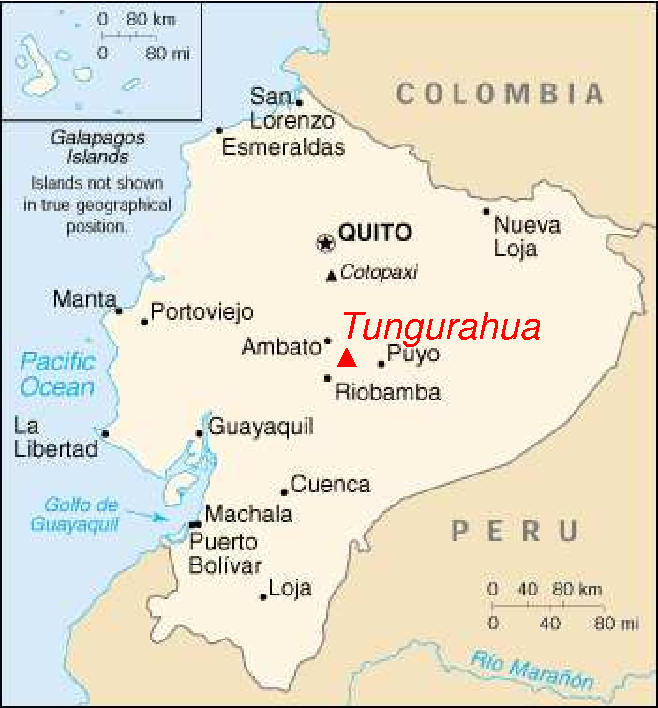
\includegraphics[width=0.7\hsize]{./figures/tungurahua.pdf}
\end{center}
\caption{\small {\bf Map showing location of Volc\'{a}n Tungurahua.}}
\label{fig-map}
\end{figure}

\subsection{Volc\'{a}n Tungurahua}

\begin{figure}[t]
\begin{center}
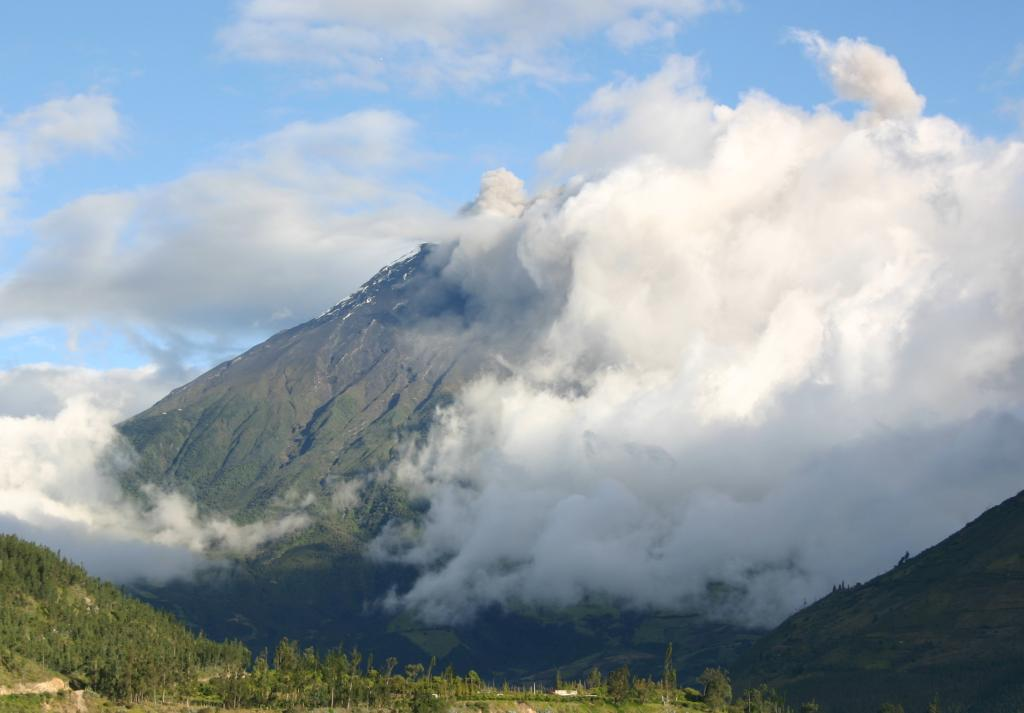
\includegraphics[width=0.9\hsize]{./figures/pics/tungurahua1.jpg}
\end{center}
\caption{\small {\bf Volc\'{a}n Tungurahua.}}
\label{fig-tungurahua}
\end{figure}

Volc\'{a}n Tungurahua (78.43$^\circ$W, 1.45$^\circ$S) is located on the
central part of the Eastern Cordillera of the Ecuadorean Andes
(Figures~\ref{fig-map}~and~\ref{fig-tungurahua}). Its current cone
has a steep flank (30-35$^\circ$ slopes) and a crater at the upper part of
its northwestern flank. Ba\~{n}os, an important tourist destination in
Ecuador with 25,000 inhabitants, is located at the foot of the volcano
close to Agoyan, one of the country's largest hydroelectric plants. Rural
communities are dispersed all around the volcano's lower flanks.

Geological studies show that Volc\'{a}n Tungurahua has produced Plinian-type
eruptions as well as at least two sector collapses ($\approx$ 13,000 
and 3,000 years b.p.~\cite{Hall99}). Since colonial times (1534), 
five eruptive cycles have occurred: 1641--1646, 1773--1781, 1886--1888,
1916--1918, and 1999--present. Generally, these eruptions were
characterized by tephra-and-ash falls covering the volcano flanks,
especially the western slopes, lahars, pyroclastic flows, and 
lava flows running down the north, west and south-western
valleys.

The current eruptive period was preceded by anomalous
seismicity first detected in 1993 by the local seismic
network~\cite{Ruiz94}.
In October 1999, after a few months of increasing
seismicity, Tungurahua emitted an ash column with incandescent blocks.
This activity led to the evacuation of more than 16,000 residents from
the surrounding areas.  As of August 2004, more than 1,900 volcanic
explosions have been recorded at Tungurahua by the Instituto Geof\'{i}sico
in Quito.  Activity has been grouped into eight eruptive cycles. The
last cycle started on May 2004 and reached its climax in June. These
eruptive periods have manifested ash emissions, and vulcanian and
strombolian activity. 

Volc\'{a}n Tungurahua is monitored by the Instituto Geof\'{i}sico of the
Escuela Politecnica Nacional (IGEPN) using a seismic network of seven
short-period stations, one broadband station, two tiltmeters, five
deformation
control lines, acoustic flow meters, and an SO$_2$-concentration
measurement system. In November 1999, a temporary microphone for
recording infrasound signals was deployed in a ridge just in front of
the volcano northwestern flank~\cite{Johnson03}.
In addition, numerous scientific campaigns, such as ours, have deployed 
temporary monitoring stations on the volcano.



\subsection{Deployment}

%My coordinate for TGUI seismometer is S01.43561, W078.46380, ELEV2889 m
%Relative to this position (0,0), my GPS tells me that:
%MOTE2 is 7 m north and 4 m east
%MOTE3 is 17 m north and 4 m west (-4 m east)
%MOTE4 is 1 m north and 2 m east

Our sensor network deployment was colocated with a wired seismic and
infrasound station used by researchers from UNC and IGEPN.  The deployment
station was located via GPS at 78.46380$^\circ$W, 1.43561$^\circ$S at
an elevation of 2889~m. 

As described previously, the aggregator node transmits data via a FreeWave
modem to a laptop acting as a base station. The laptop was kept at the 
volcano observatory operated by IGEPN, which is located 9~km away from 
the monitoring station. The observatory is in a valley with direct
line-of-sight to the monitoring station on the volcano.
A pair of 9~dBi 900~MHz Yagi antennas (Figure~\ref{fig-infrasound}(c)) were used to
establish connectivity between the two FreeWave modems. The GPS receiver
and FreeWave modem were powered by a 12~V car battery (smaller lead-acid
batteries were used for testing but are disallowed on commercial air
flights). All other nodes were powered by 2~AA batteries and operated
continuously during the 54-hour deployment.

The aggregator node, GPS receiver, FreeWave modem, Yagi antenna, and
car battery were placed at the foot of a tree. One of the infrasonic
nodes was placed about 1~m above ground in the same tree. Another node was
placed 6.3~m away in a second tree, while the third node was placed
10.7~m away on a tree stump. Infrasound nodes were elevated in trees both to
improve radio reception and to minimize molestation by cows grazing nearby.
The terrain at this location was fairly steep with a large amount of
vegetation, making it difficult to select locations further away from the
aggregator node.

% Placement of sensor nodes at Juive station
% Colocation with wired seismic and acoustic array
% Use of long-distance Yagi antenna, car batteries

\subsection{Data analysis}

\begin{figure}[t]
\begin{center}
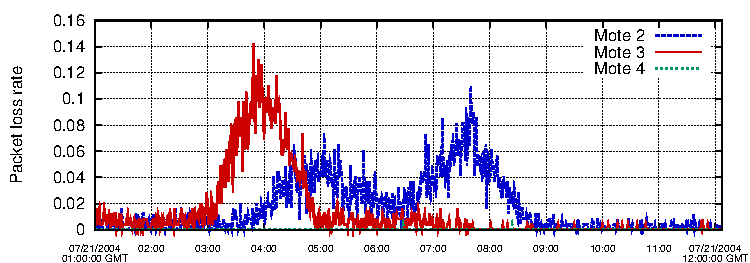
\includegraphics[width=1.0\hsize]{./figures/loss/lossrate.pdf} \\
\vspace{0.1in}
\begin{small}
\begin{tabular}{|llll|} \hline
{\em Mote} & {\em Received pkts} & {\em Lost pkts} & {\em loss rate} \\ \hline
{\em node 2} & 19470100 & 555696 & 2.77\% \\
{\em node 3} & 19039684 & 995416 & 4.96\% \\
{\em node 4} & 19584438 & 290525 & 1.46\% \\ \hline
\end{tabular}
\end{small}
\end{center}
\caption{\small {\bf Packet reception and loss statistics.}
{\em The graph shows packet loss rate, averaged over one-minute intervals,
for an 11-hour trace. Mote~4 exhibited negligible losses during this
time. The table summarizes packet loss over the
entire 54-hour deployment.}}
\label{fig-lossrate}
\end{figure}

We logged over 54~hours of continuous data from the sensor
network. Analyzing this raw data presented a number of challenges.
Although the infrasound nodes use a retransmission scheme to improve
reliability, a large number of packets are missing from the recorded
dataset. On several occasions, the FreeWave modems would experience
short dropouts of several seconds, causing data from all nodes to be
lost. In addition, GPS timestamp messages from the GPS receiver may not
have been received at the basestation, although the infrasound motes may
have received the message. Finally, on a number of occasions,
duplicate packets were recorded, most likely due to a lost acknowledgment
and redundant retransmission.  
Before registering the data to a common
timebase as described in Section~\ref{sec-regression}, it was necessary to
``clean up'' the raw logs by accounting for lost and duplicate packets.

The loss rate for each node varied during the deployment.
Figure~\ref{fig-lossrate} shows the loss rate, averaged over
one-minute intervals, for an 11-hour trace. We believe that the
gradual variation in loss is due to weather conditions (e.g., rain)
affecting radio transmission, although it is possible that temperature
fluctuations (heating and cooling of components in the Pelican cases)
may have contributed to this effect as well.
Mote~4 experienced very low loss, due 
to its positioning with a clear line-of-sight to the receiver.
Note that Mote~2, despite being located in the tree above the receiver,
experienced somewhat higher losses, probably due to antenna orientation.
Figure~\ref{fig-lossrate} summarizes the packet loss rate for each 
of the motes during the entire deployment.

% Overall statistics (total amount of data, how many eruptions)
% Statistics on lost packets, dup packets, out of order packets, over time
% Details on time regression (from Hassan's scripts)
% How much error in the regression

% Show a figure with an example explosion
% (also with Mario's seismic and acoustic data alongside)

% Look at some explosions and see if time delay between arrivals is
% consistent

\begin{figure*}[t]
\begin{center}
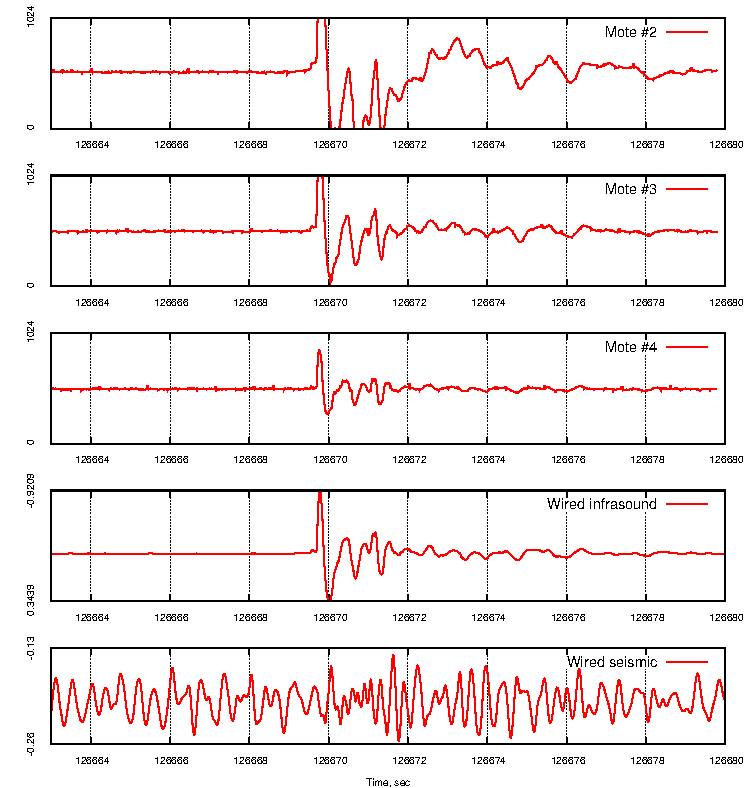
\includegraphics[width=0.7\hsize]{./figures/explosion/explosion.pdf}
\end{center}
\caption{\small {\bf Example infrasonic and seismic data from an
explosion at Tungurahua.} {\em The top three graphs show the signal
recorded by our wireless infrasonic sensor network
(July 21 2004 at 11:11:00 GMT).
The bottom two graphs show infrasonic and seismic signals from the
same explosion recorded by a colocated wired station.}}
\label{fig-explosion}
\end{figure*}

Through visual inspection of the time-regressed logs, we manually
verified well-correlated infrasonic signals from nine separate explosions 
recorded during our deployment. The frequency of explosions varied
greatly, with inter-explosion times ranging from 1~hour to over 24~hours.
Data recorded by our sensor array during an example explosion is 
shown in Figure~\ref{fig-explosion}.
Infrasonic and seismic data from the colocated wired station is shown
for comparison. As the figure shows, the wireless array demonstrates
very good correlation with wired station.
Note that the seismic signal precedes the acoustic by
several seconds due to its faster propagation speed.


\section{Distributed Event Detection}
\label{sec-distrib}

Our initial deployment on Volc\'{a}n Tungurahua was small enough
that it was possible to transmit continuous signals from each of the
nodes. However, such an approach is not feasible for larger arrays deployed
over longer periods of time. We are planning to deploy a much larger
(approximately 30 node) sensor array on Tungurahua within the next 
8-12~months. To save bandwidth and energy, it is desirable to avoid
transmitting signals when the volcano is quiescent. In this section,
we describe a distributed event detector that only transmits
well-correlated signals to the base station.

%We had several advantages when approaching the general network triggering
%problem.  One stems from the eruption frequency of volcanos like Tungurahua,
%which are considered highly active when erupting merely dozens of times per
%day.  This event frequency allows time between events during which data
%collection and transmission can occur.  A second significant advantage we had
%was the data that we collected at Tungurahua.  Possessing a large amount of
%actual data collected at a real volcano on our hardware platform allowed us
%to test certain portions of our distributed event detector in simulation
%retaining total confidence in the results.

\subsection{Distributed Detector Design}

Our distributed detector uses a decentralized voting process to measure
signal correlation among a group of nodes.  Each node samples data
continuously at 102.4~Hz and buffers a window of acquired data while
running a local event detection algorithm.  When the local event detector
triggers, the node broadcasts a vote message. If any node receives
enough votes from other nodes during some time window, it initiates
global data collection by flooding a message to all nodes in the
network. Note that in this approach, voting uses local radio
broadcast, while data collection is initiated using a global flood.
Our expectation is that in a typical deployment, each node will 
have multiple neighbors within radio range with which it can compare
votes using local broadcast only. 

To reduce radio contention during data collection, we use a token-based
scheme for scheduling transmissions. Upon initiating global data
collection, the first node (ordered by node ID)
transmits its complete buffer of data to the base station, performing
retransmissions for any lost packets. Once the complete buffer has been
transmitted, the node broadcasts a message indicating that the next
node in the numeric sequence should transmit its buffer. If a node
does not hear the token exchange (or has failed), the base station will
flood the network with a data request after a timeout period, ensuring
forward progress.

\subsection{Local Detector Design}

Our design decouples the distributed voting scheme from the specific
local event detection algorithm used, allowing us to explore different
approaches. Figure~\ref{fig-explosion} shows a typical infrasonic
wave.  Designing a local event detector for this kind of waveform is
straightforward, although some tuning is required to minimize false
positives (which may trigger data collection for uncorrelated signals)
and false negatives (which may cause true explosions to be missed).

We have implemented two local event detectors: a threshold-based detector
and an exponentially weighted moving average (EWMA)-based detector. The
threshold detector is triggered whenever a signal rises above one
threshold, $T_\mathrm{hi}$, and falls below another, $T_\mathrm{lo}$,
during some time window $W$.  Because this detector relies on absolute
thresholds, it is sensitive to the particular microphone gain on each
node. It is also susceptible to false triggering due to spurious
signals, such as wind noise, although the voting scheme described above
mitigates this effect.

The EWMA detector calculates two moving averages with different
gain parameters, $\alpha_\mathrm{short}$ and $\alpha_\mathrm{long}$,
representing both short-term and long-term averages of the 
signal. For each ADC sample, each moving average is calculated as:
\[
\mathit{average} = \alpha \cdot \mathit{sample} + (1 - \alpha) \mathit{average}
\]
For our analysis below, we use $\alpha_\mathrm{short} = 0.05$
and $\alpha_\mathrm{long} = 0.002$.
For each new sample, the detector compares the ratio of the two
averages. If the ratio exceeds some threshold $T$ (i.e., the short-term 
average exceeds the long-term average by a significant amount), 
the detector is triggered. This detector is less affected by 
the sensitivity or bias of individual sensor nodes. Because a large
signal will cause the detector to trigger for multiple successive
samples, we suppress duplicate triggers over a window of 100~samples.

\begin{figure}[t]
\begin{center}
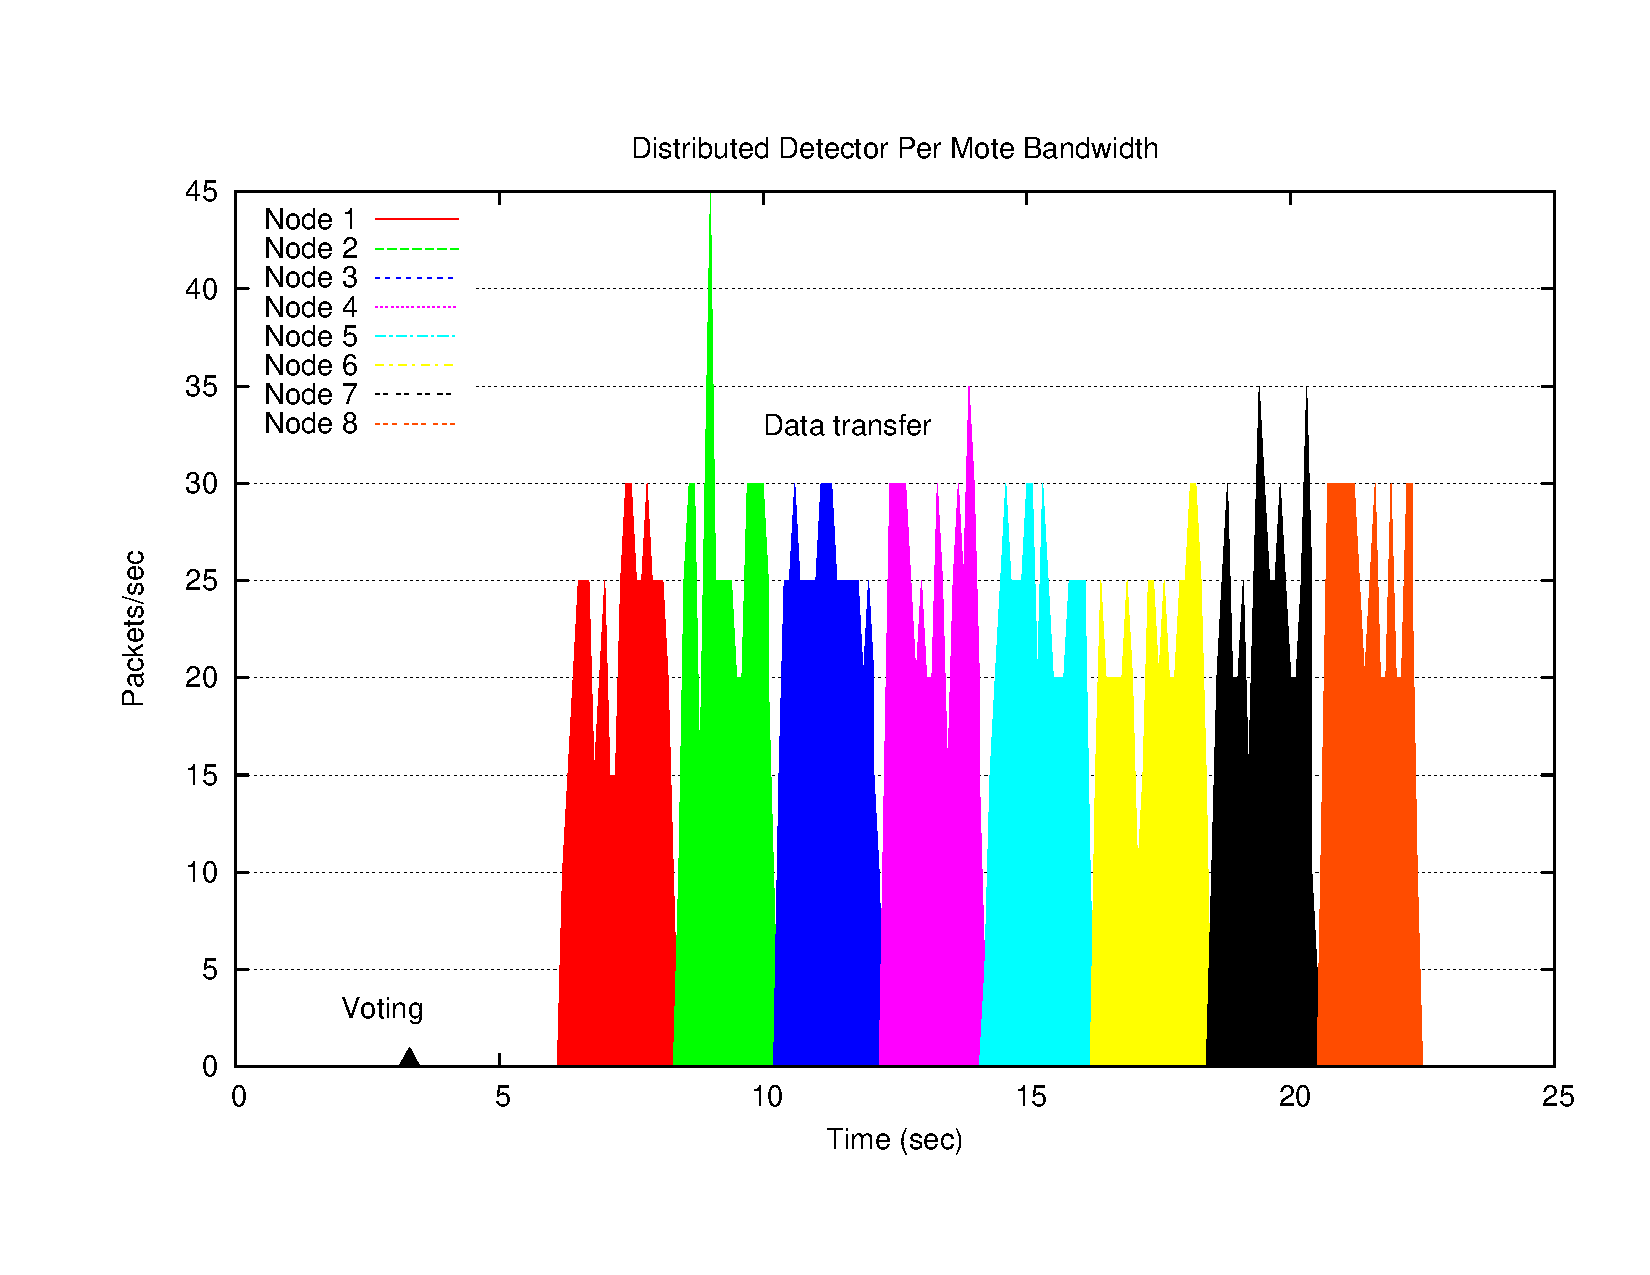
\includegraphics[width=0.9\hsize]{./figures/DD/bandwidth.pdf}
\end{center}
\caption{\small {\bf Distributed detector network bandwidth
consumption.} {\em Values are shown as packets per second. The 
voting and round-robin data collection phases are clearly visible.}}
\label{fig-packetssec}
\end{figure}

\section{Evaluation}
\label{sec-evaluation}

We implemented the distributed event detector in TinyOS and tested it
on an array of 8 Mica2 nodes in our lab.  The infrasonic signals used
to trigger the array were produced by decisively closing the lab door, 
which closely mimics infrasonic signals produced by a volcano.  Since the
lab experiments were not intended to evaluate the accuracy of the local
detector we exploited the lack of wind noise in the lab and deployed the
simple threshold detector described above.  Because we were only able
to deploy 4~nodes with infrasonic sensor boards, the voting thresholds were
adjusted accordingly.  Although only 4~nodes participated in the voting
process, data was still collected from all 8~nodes, the remaining four
equipped with standard Mica2 sensor boards (which are not sensitive 
enough to detect infrasound).

\subsection{Energy usage}

Figure~\ref{fig-continuouspowerconsumption} shows the power consumption 
of a node running the original continuous data-collection code.
For comparison, Figure~\ref{fig-ddpowerconsumption} shows the power
consumption of the distributed event detector. Each node exhibits
a baseline current draw of about 18~mA. The continuous sampling code
experiences spikes up to 36~mA during radio packet transmissions
every 4~Hz, while the distributed detector only experiences these
spikes while transmitting votes and (for correlated signals) data
transmission to the base station. 

Assuming a constant 3~V supply voltage, under the continuous sampling model 
the total power consumption over a time interval $t$ is roughly:
\[
   P_c = 3 \cdot 18 + \rho_\mathrm{tx} P_\mathrm{tx}  \mathrm{mW}
\]
where $P_\mathrm{tx}$ is the power required to transmit a single
packet, and $\rho_\mathrm{tx}$ is the rate of transmission, 
approximately 4~Hz.
For the distributed detector, the power consumption is:
\[
   P_d = 3 \cdot 18 + \rho_\mathrm{vote} P_\mathrm{tx} +
     \rho_\mathrm{send} P_\mathrm{tx} n
\]
where $\rho_\mathrm{vote}$ is the local voting rate,
$\rho_\mathrm{send}$ is the rate at which correlated signals are
transmitted to the base station, and $n$ is the number of packets in the
local window to transmit. 

On the Mica2, the time to transmit a single packet is approximately
20~ms, so $P_\mathrm{tx} = 3 \cdot 20 \mathrm{ms} \cdot 36 \mathrm{mA} =
2.16$ mW. To transmit a buffer of 1500 samples with 25 samples/packet,
$n = 60$ packets.

Assuming that nodes detect a correlated signal every 1/2 hour, 
and locally vote at twice this rate (i.e., 100\% false positive event
detection), we have
\begin{eqnarray*}
  P_c &=& 3 \cdot 18 + 2.16 / 4 = 54.54 \mathrm{mW} \\
  P_d &=& 3 \cdot 18 + 2.16 / 900 + 50 (2.16 / 1800) \\
      &=& 54.062 \mathrm{mW}
\end{eqnarray*}
for a savings of 0.48 mW. Note that in both cases, power usage is 
dominated by the 18~mA baseline current consumption. By employing careful 
duty cycling of the CPU and radio in between sampling periods, energy usage
could be reduced further, and we intend to explore this as future work.
% Lifetime: (2.850 A-hours in a battery) / (Power / 3V) = # hours

\subsection{Bandwidth usage}

\begin{figure}[t]
\begin{center}
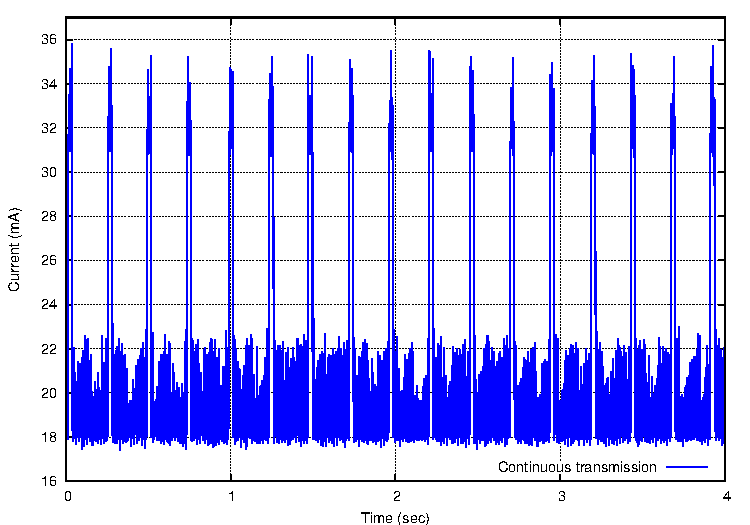
\includegraphics[width=0.9\hsize]{./figures/DD/mdw/continuous.pdf}
\end{center}
\caption{\small {\bf Power consumption of the original 
continuous data collection code.} 
{\em The baseline power consumption is about 18~mA, while
high-frequency spikes up to 22~mA are caused by ADC sampling.
The 4~Hz spikes are caused by radio 
packet transmissions. Due to CSMA backoff these transmissions
are not equally spaced.}}
\label{fig-continuouspowerconsumption}
\end{figure}

\begin{figure}[t]
\begin{center}
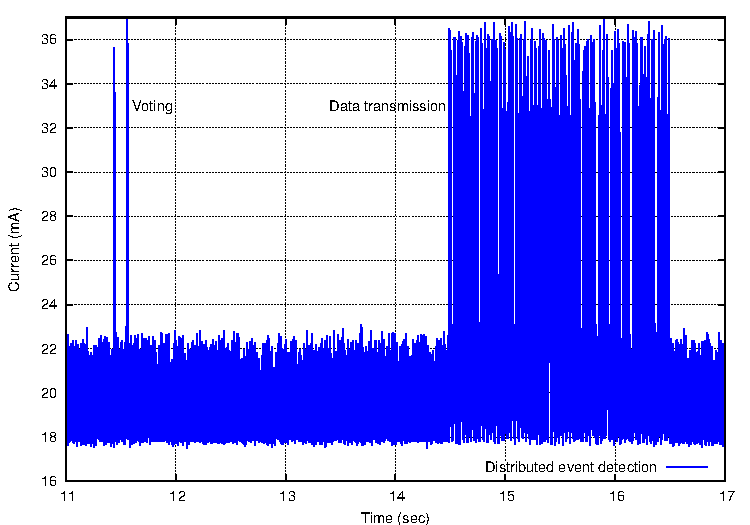
\includegraphics[width=0.9\hsize]{./figures/DD/mdw/dd.pdf}
\end{center}
\caption{\small {\bf Power consumption of the distributed event 
detection code.} {\em Overall power consumption is limited to 
sampling, while radio transmissions occur during voting and
data transfer phases.}}
\label{fig-ddpowerconsumption}
\end{figure}


Figure~\ref{fig-packetssec} shows the number of radio messages 
transmitted by the sensor array during the detection
of an event, clearly showing the voting and data collection phases.
The delay between the decision to collect data and the onset of the data
collection phase allows the nodes to center the event in their buffers.  As
shown on the graph, approximately 16~sec are required to complete data
recovery from 8 nodes in our current distributed detector. Note that we do
not currently use any compression or larger data packet sizes, 
both of which would improve transfer speed. This latency scales
linearly with the number of nodes in the array and the size of the sample
buffer on each node. The total
number of nodes in the network is bounded only by the total amount of
time to transfer complete signals to the base station, which is far
less than the expected frequency of eruptions. Even if this were not 
the case, nodes could readily log multiple events to EEPROM for later
transmission.

In contrast, the continuous sampling scheme requires each node to
transmit one packet every 1/4~sec, consuming $(n \times 4 \times 32)$
bytes/sec of bandwidth (counting application payload only), 
where $n$ is the number of nodes. 
We have benchmarked the radio performance of the Mica2 node which can
achieve roughly 7~Kbps from a single transmitter. Assuming perfect
channel sharing, a single radio hop, and no packet loss, we can optimistically 
support up to 7~nodes in this configuration. 
We have benchmarked the CC2420 802.15.4 radios on the Telos mote as 
capable of achieving about 22.5~Kbps (using the standard TinyOS MAC layer
and packet size), allowing up to 25~nodes in a single radio hop. 
However, with this many nodes it would be necessary to spread the array
over a larger area, requiring multihop communication which reduces
available bandwidth.

\subsection{Detector Accuracy}

\begin{figure*}[t]
\begin{center}
\begin{tabular}{|llllll|} \hline
{\bf Parameters} & {\em Total votes} & {\em Total events} & {\em True events} & {\em False positives} & {\em False negatives} \\ \hline
\multicolumn{6}{|c|}{\em Threshold detector} \\ 
100/900/2 & 2187 & 7 & 6 & 1 & 3 \\ 
200/800/2 & 2918 & 11 & 8 & 3 & 1 \\ 
300/700/2 & 4486 & 32 & 9 & 23 & 0 \\ 
400/600/2 & 9098 & 246 & 9 & 237 & 0 \\ \hline
100/900/3 & 2191 & 3 & 3 & 0 & 6 \\ 
200/800/3 & 2931 & 4 & 4 & 0 & 5 \\ 
300/700/3 & 4624 & 10 & 7 & 3 & 2 \\ 
400/600/3 & 11390 & 66 & 9 & 57 & 0 \\ \hline
\multicolumn{6}{|c|}{\em EWMA detector} \\ 
1.5/2 & 575 & 14 & 9 & 5 & 0 \\ 
1.75/2 & 444 & 8 & 7 & 1 & 2 \\ 
2.0/2 & 374 & 7 & 7 & 0 & 2 \\ \hline
\end{tabular}
\end{center}
\caption{\small {\bf Distributed event detector accuracy.} 
{\em For the threshold detector, the {\em Parameters} column is 
in the form {\em low/high/thresh},
where {\em low} is the low-signal threshold, {\em high} is the
high-signal threshold, and {\em thresh} is the number of nodes that
must report a local event before a correlation is made.}
For the EWMA detector, the format is {\em ratio/thresh},
where {\em ratio} is the ratio of low EWMA to high EMWA
that triggers a local event, and {\em thresh} is the voting threshold, 
as above.}
\label{fig-dd-accuracy}
\end{figure*}

The accuracy of the two local event detector algorithms is presented in
Figure~\ref{fig-dd-accuracy}. For this experiment, we fed the detectors
with the complete trace of data recorded on Tungurahua. Recall that
there are 9~known explosions in this data over a 54~hour period.
For each set of parameters, the total number of votes (potential local
events) is shown, along with the number of correlated events resulting in
global data collection. We manually verified each of the reported events
as true explosions or false positive detections.

As expected, as the local detector becomes more selective, fewer voting
rounds are initiated, although not all of the known explosions are
detected. Increasing the number of votes required to trigger global data
collection further reduces the sensitivity of the distributed detector.
It is important to keep in mind that even with a large number of false
positives, the distributed event detector saves significant bandwidth
over continuous sample transmission.



\section{Conclusions}
\label{sec-conclusions}


%%%%%%%%%%%%%  THIS IS WHERE THE BIBLIOGRAPHY GOES %%%%%%%%%

\def\baselinestretch{0.92}
\begin{footnotesize}
\setlength{\itemsep}{2in}
\bibliographystyle{IEEEtran} \bibliography{ewsn,johnson}
\end{footnotesize}

\end{document}
